\begin{frame}{Textual macro languages}
    \begin{itemize}
        \item Textual Macros are macros that directly affect the text of the 
            programming language without knowing about or dealing with the 
            meaning of the language \emph{e.g.} C preprocessor\cite{macrosibm}. 

        \item Allows you to write small Domain Specific Languages(DSLs).

        \item Some times these small DSLs are easier to write and maintain than
            the same construction in the target language.

        \item Textual macros affect the text of the program without dealing 
            with semantics.
    \end{itemize}
\end{frame}

\begin{frame}{C/C++ \emph{\#define} Macro}
    \begin{itemize}\addtolength{\itemsep}{1\baselineskip}
        \item Textual macro expansion.

        \item Basic way to do basic metaprogramming.
    \end{itemize}
\end{frame}

\begin{frame}{C preprocessor SWAP}
    \begin{center}
        \begin{tikzpicture}[]
            \node[] at (0mm,0mm){
                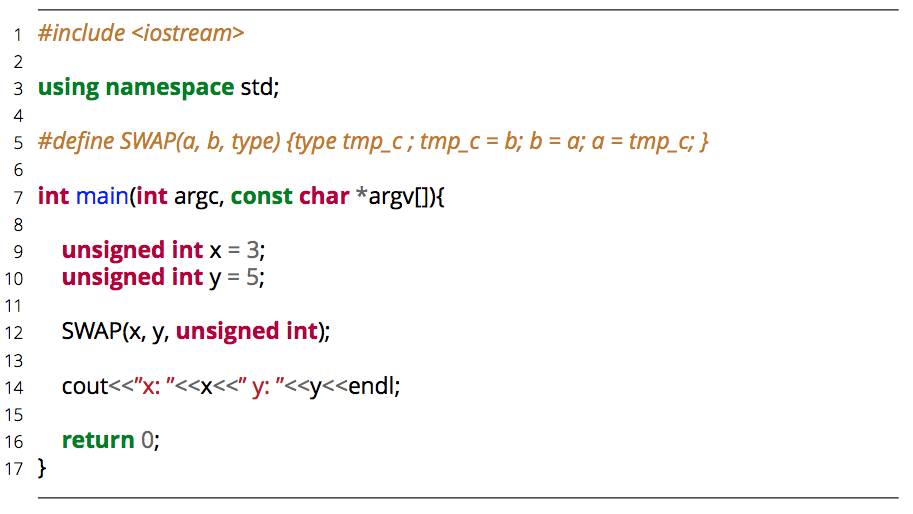
\includegraphics[height=60mm]{/Users/lalanne/MyCode/GitHubProjects/MetaTalk/figures/swap.png}\hspace{5mm}
            };
        \end{tikzpicture}
    \end{center}
\end{frame}

\begin{frame}{C preprocessor SWAP}
    \begin{center}
        \begin{tikzpicture}[]
            \node[] at (0mm,0mm){
                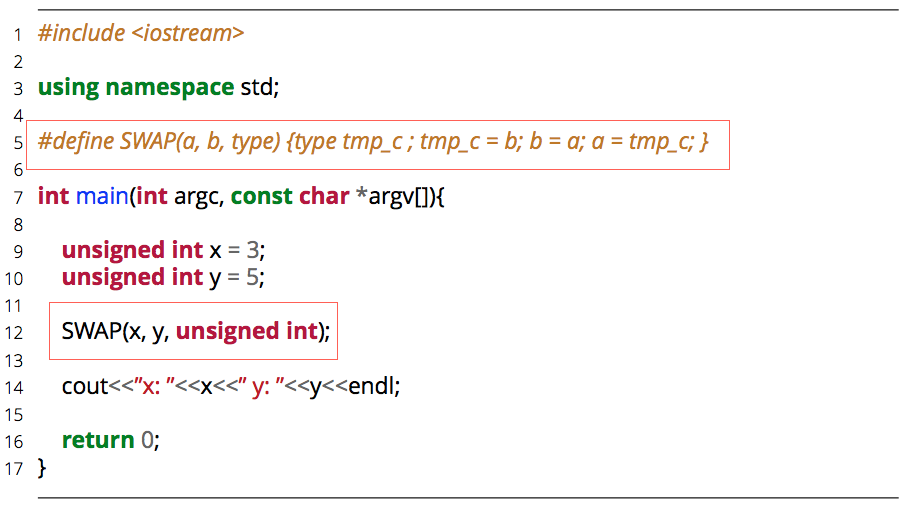
\includegraphics[height=60mm]{/Users/lalanne/MyCode/GitHubProjects/MetaTalk/figures/swap1.png}\hspace{5mm}
            };
        \end{tikzpicture}
    \end{center}
\end{frame}

\begin{frame}{C preprocessor SWAP expanded}
    \begin{center}
        \begin{tikzpicture}[]
            \node[] at (0mm,0mm){
                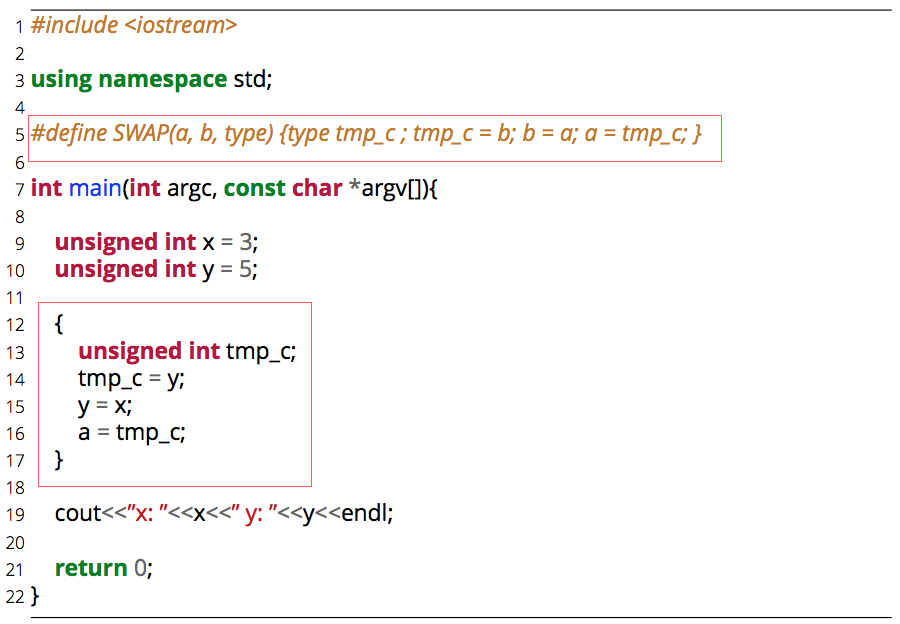
\includegraphics[height=70mm]{/Users/lalanne/MyCode/GitHubProjects/MetaTalk/figures/swapexp1.png}\hspace{5mm}
            };
        \end{tikzpicture}
    \end{center}
\end{frame}

\begin{frame}{C preprocessor SWAP expanded}
    \begin{center}
        \begin{tikzpicture}[]
            \node[] at (0mm,0mm){
                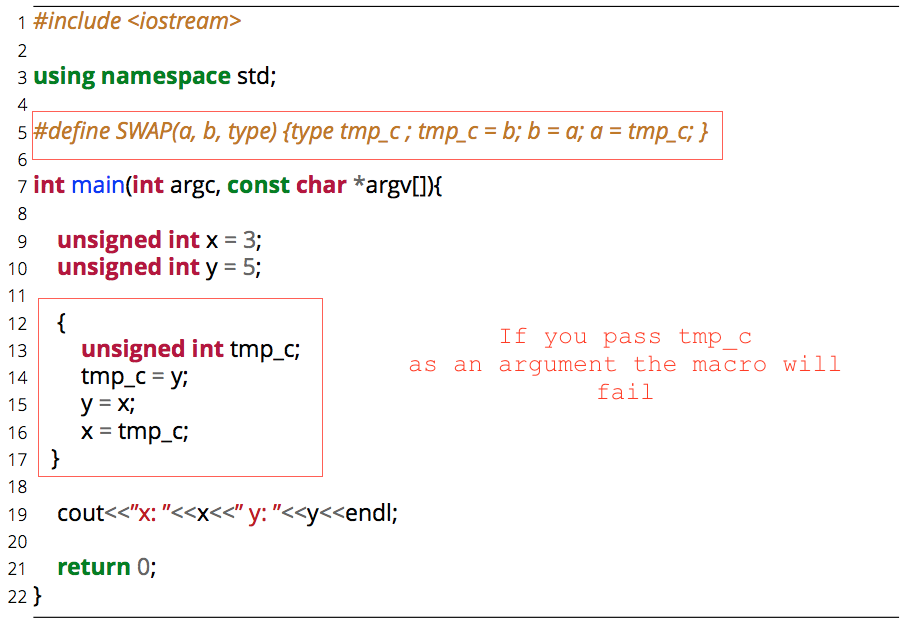
\includegraphics[height=70mm]{/Users/lalanne/MyCode/GitHubProjects/MetaTalk/figures/swapexp2.png}\hspace{5mm}
            };
        \end{tikzpicture}
    \end{center}
\end{frame}


\begin{frame}[fragile]{C preprocessor MIN}
\inputminted[mathescape,
           linenos,
           numbersep=5pt,
           frame=lines,
           bgcolor=White,
           fontsize=\scriptsize,
           linenos,
           framesep=2mm]{c++}
           {/Users/lalanne/MyCode/GitHubProjects/MP_Talk/macro_min.cpp} 
\end{frame}

\begin{frame}[fragile]{C preprocessor MIN}
\inputminted[mathescape,
   linenos,
   numbersep=5pt,
   frame=lines,
   bgcolor=White,
   fontsize=\scriptsize,
   linenos,
   framesep=2mm]{c++}
   {/Users/lalanne/MyCode/GitHubProjects/MetaTalk/src/code/macro_min_fail.cpp} 
\end{frame}

\begin{frame}[fragile]{C preprocessor MIN}
\inputminted[mathescape,
   linenos,
   numbersep=5pt,
   frame=lines,
   bgcolor=White,
   fontsize=\scriptsize,
   linenos,
   framesep=2mm]{c++}
   {/Users/lalanne/MyCode/GitHubProjects/MetaTalk/src/code/macro_min_should.cpp} 
\end{frame}

\begin{frame}[fragile]{C preprocessor MIN}
\inputminted[mathescape,
   linenos,
   numbersep=5pt,
   frame=lines,
   bgcolor=White,
   fontsize=\scriptsize,
   linenos,
   framesep=2mm]{c++}
   {/Users/lalanne/MyCode/GitHubProjects/MetaTalk/src/code/macro_min_res.cpp} 
\end{frame}

\begin{frame}[fragile]{C preprocessor MIN}
\inputminted[mathescape,
   linenos,
   numbersep=5pt,
   frame=lines,
   bgcolor=White,
   fontsize=\scriptsize,
   linenos,
   framesep=2mm]{c++}
   {/Users/lalanne/MyCode/GitHubProjects/MetaTalk/src/code/macro_min_ext.cpp} 
\end{frame}

\begin{frame}{The MIN case}
    \begin{itemize}\addtolength{\itemsep}{2\baselineskip}
        \item Necessary parenthesis (operator precedence), what happen if you 
            do \emph{MIN(27, b=3)}.

        \item When one of the arguments is a function is going to be call twice. 
            (performance, duplicated calculation). Worst when the function
            contains side effects(printing).
    \end{itemize}
\end{frame}

\begin{frame}{Advantages}
    \begin{itemize}\addtolength{\itemsep}{1\baselineskip}
        \item Function call too much overhead for this simple operation (myth).

        \item With big types you end up using pointers(aliasing).
            {\color{red}mmmm check!}

        \item Different functions for different types.
    \end{itemize}
\end{frame}

\begin{frame}{Disadvantages}
    \begin{itemize}\addtolength{\itemsep}{1\baselineskip}
        \item C/C++ preprocessor allow limited arguments for Macros.

        \item You do not get any type of type safety.
            {\color{red} some kind of example of this}

        \item Its get very messy when you combine Macros with expressions.
    \end{itemize}
\end{frame}

